\documentclass[12pt]{article}
\usepackage{wkrpt}
\begin{document}


\title{Evaluation of Synchronous and Asynchronous Programming techniques in Ecommerce Application}
{
	Minted LLC.\\
	San Francisco, CA 94111
}
{
	\textbf{Prepared by}\\[2ex]
	
	Daiwei Fan\\
	Student ID: 20458752\\
	User ID: d3fan\\
	4A Software Engineering\\
	May 1, 2016
}


\letter{Evaluation of Synchronous and Asynchronous Programming techniques in Ecommerce Application}{third}{3B}{Minted LLC.}
{
	\noindent
	Daiwei Fan\\
	\#48, 461 Beechwood Place\\
	Waterloo, ON\\
	N2T 2N8
}
{
	Minted is a ecommerce platform that sells customizable arts and designs. Their main product include wedding invitations, digital invitations, uniquely designed stationary items etc. I decided to write this report based on the various concurrent programming techniques used in Minted's ecommerce funnel.
}
{
	The following report performs an evaluation on the use of synchronous and asynchronous techique used in different phases of the ecommerce funnel. The correct usage of technique is the interest of many parties in the company. My report will be used as a minor suggestion to the engineering team who makes the final decision of code refactoring.
}
{
	I would like to thank my mentor Linus Mixson, co-worker James Wu and devops engineer Patrick Gilbert, all of whom provided valuable background knowledge and priceless guidance over the course of my internship.
}
{
	Daiwei Fan\\
	Student ID: 20458752\\[2ex]
	Encl.
}


\tocsection{Executive Summary}




\newpage

\tableofcontents
\newpage
\listoffigures
\newpage
\listoftables
\newpage


\pagenumbering{arabic}
\section{Introduction}

Minted is an online marketplace of independent artists and designers. The company crowdsources art and graphic design through monthly challenges. The public votes for the winning entries, and Minted produces the winning work as stationery, wall art, and decor.\cite{telusComp}. In October 2014, Minted was named #5 on LinkedIn's 10 Bay Area startups that are most in demand by local techies. In January 2014, I was assigned to the VIP room to implement a web service that mainly contains a drug claim searching and benefit management feature. This particular feature allows different levels of users such as patient, insurer and pharmacist to access the patient's record of drug claims and payments. After a certain amount of designing and coding, it came to the point where some basic testing for the code was necessary. I believe that even elementary testings should be carefully designed for future documentation and reproduction. \\

Functionality testing has always been one of the most important tasks in the quality assurance (abbreviated as QA) process. All companies are working to discover a testing method which is able to cover all sources of error, requires minimal human effort and consumes least amount of time. It is especially important for Telus Health, a company which has adapted the Agile software development system, to have a highly efficient QA process in order to accommodate the fast pace of the system. At Telus, agile development is structured as series of “sprint cycles.” Every aspect of the development process, including technical requirements, design etc., are continually revisited throughout the lifecycle of the project. As a consequence, a series of developing and testing will take place. As illustrated in Figure 1, the testing phase appears on a intense frequency, which results in many high demands on the tests' quality, efficiency etc. These demands will be considered as criteria to evaluate a testing approach later on in the report.\\

\begin{figure}[ht!]
\centering
\includegraphics[width=12.5cm,height=12.5cm,keepaspectratio]{img/agile.png}
\caption{Agile development workflow}
\label{overflow}
\end{figure}

This report provides an evaluation of three functionality testing methods, assessing their 
suitability to the VIP room web service. You will first be introduced to the VIP room work flow. Then, the three approaches for testing will be explained and compared in detail. Comparisons will be made among various criteria and will be finalized using the Decision Matrix Analysis. Finally, the report summarizes the results of the analysis, draws 
conclusions, and makes a recommendation. The reader is expected to have reasonable background in web service development. Basic knowledge in the Extensible Markup Language (XML)would also help the reader quickly understand one of the approaches. Other technology and terminologies used in this report will be explained on their first appearance.\\



\newpage

\section{Problem Specification}
\subsection{Background}
The web application uses Apache Maven as its build manager and Apache Tomcat as server. It utilizes the traditional three-tier architecture. Figure 2 depicts the sequence diagram of a three-tier web service workflow:

\begin{figure}[ht!]
\centering
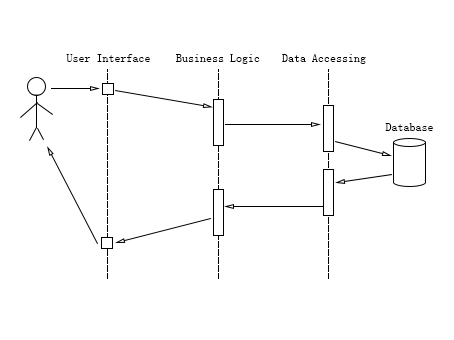
\includegraphics[width=12cm,height=12cm,keepaspectratio]{img/three_tier.jpg}
\caption{three-tier web service sequence diagram}
\label{overflow}
\end{figure}


\subsection{Options}
The three testing approaches sends data to different part of the flow.
\subsubsection{Manual testing from User Interface}
The most naive method is to manually enter input data on the User Interface (UI) \\
		
\begin{figure}[ht!]
\centering
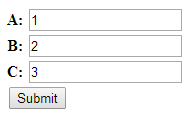
\includegraphics[width=5cm,height=5cm,keepaspectratio]{img/ui.jpg}
\caption{input from simple UI}
\label{overflow}
\end{figure}

\subsubsection{Simple Object Accessing Protocol (SOAP)}
	This method uses the Simple Object Accessing Protocol. "SOAP is a lightweight protocol for exchange of information in a decentralized, distributed environment."\cite{soap} It wraps the input data in an envelope and sends it as a request directly to the business layer. A soap request template is populated based on a file written in Web Services Description Language (WSDL). This file can be generated from a Java Class containing business logic. In most cases this Class is the controller or entrance to the business layer. The following is a screen shot of a SOAP client called “SoapUI”:
	
\begin{figure}[ht!]
\centering
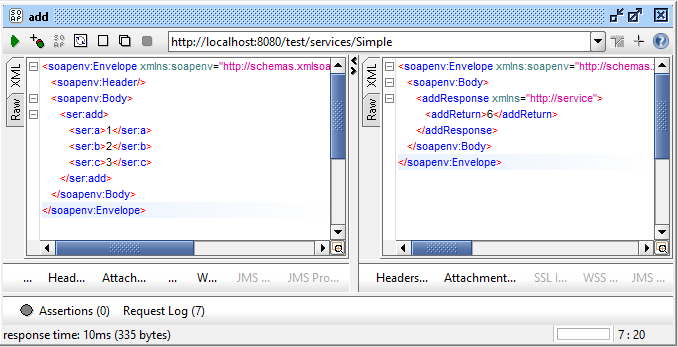
\includegraphics[width=15cm,height=15cm,keepaspectratio]{img/soapui.jpg}
\caption{SoapUI request/response}
\label{overflow}
\end{figure}

The XML message on the left is a simple request containing three parameters and the one on the right is its response. This request template is populated from WSDL file (shown in appendix) generated by the following Java Class:\\

\begin{lstlisting}
// Simple.java
public class Simple {
	public int add(int a, int b, int c){
		return a + b + c;
	}
}

\end{lstlisting}

In short, SOAP can be used to replace the web service's native UI and take its role in terms of sending data to business layer and receive response from it.

\subsubsection{Unit Testing}
This approach uses a popular testing method called unit testing. “The primary goal of unit testing is to take the smallest piece of testable software in the application, isolate it from the remainder of the code, and determine whether it behaves exactly as you expect. Each unit is tested separately before integrating them into modules to test the interfaces between modules.”\cite{unit} Regarding the aspect of directing data, unit testing sends data to almost everywhere. A good analogy is that when launching a rocket. Every engineer is assigned to inspect the status of one tiny part of the rocket. Hundreds of them work together and simultaneously to finish inspecting the entire rocket. The following code is a JUnit test case:\\
\begin{lstlisting}
// SimpleTest.java
import static org.junit.Assert.*;
import org.junit.Test;

public class SimpleTest {
	@Test
	public void test() {
		//Class Simple is being tested
		Simple tester = new Simple();
		//check if 1 + 2 + 3 returns 6
		assertEquals("1 + 2 + 3 must be 6", 6, tester.add(1,2,3));
	}
}
\end{lstlisting}
\newpage

\section{Comparison}
It is not doubt that efficiency plays an important role when it comes to judging which approach is the best. Therefore all factors that influence the efficiency of the test should be analysed separately.  The three approaches will be compared against each of these criteria. And in the end the criteria will be weighed based on their level of importance to produce one final sum for each approach.\\
\subsection{Time}
This subsection measures the average amount of time to run one single test. All three approaches will use the exact same inputs. The data used will be typical for VIP room clients. Due to confidentiality and copyright, the input data can only be briefly described as:  It contains six mandatory fields and seven optional fields. Three of the mandatory fields are numerical fields and the rest are alphabetical. All seven optional fields are alphabetical fields.\\

Five sets of input was selected with each taking notably different amount of time when tested. Each set is tested three times on each approach to increase precision and the result is shown in Figure 5 (All values take the unit of a millisecond):\\


\begin{figure}[ht!]
\centering
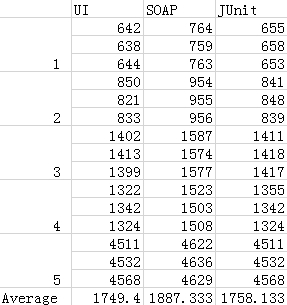
\includegraphics[width=6cm,height=6cm,keepaspectratio]{img/timeTable.jpg}
\caption{Time taken by different approaches}
\label{overflow}
\end{figure}


Figure 6 illustrates the average time taken every test case:\\

\begin{figure}[ht!]
\centering
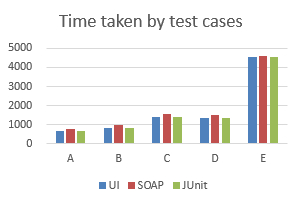
\includegraphics[width=9cm,height=9cm,keepaspectratio]{img/timeGraph.jpg}
\caption{Time taken by test cases}
\label{overflow}
\end{figure}

The graph shows that all three approaches finish all test cases in the same time frame with SOAP taking the longest and JUnit taking the least. This result is reasonable since the amount of time that runtime execution takes is dominant in the values displayed on the graph. At the mean time, the SOAP protocol wraps input data in an envelope when sending and checks the output with assertions and validations. This can explain the fact that it is taking longer than the others. Please note that this subsection does not measure the amount of time for quality analysts to enter the data when using the three approaches. This justified in the next two subsections. \\


\subsection{Automation}
Automation is the most popular topic among quality analysts who seek to improve their testing. Testing automation is a technique that boosts efficiency and reduces human labour. A large number of test cases are controlled by the system and run against the web application automatically when a test command is generated by the tester or when the application is built.\\

The first approach is the least automation friendly approach, considering that data is entered from the UI. Although it is possible using a language such as Python, this is not encouraged or practically viable. The reason is that VIP room is an enterprise web application with thousands of customers. The security layer that wraps the application redundantly checks if the data is entered by some artificial intelligence to prevent brute force security penetration. Therefore automated testing is not feasible for this approach.\\

The possibility for automated SOAP testing solely depends on the software used. Some light weight SOAP software (or web client) does not have automation features. However in SoapUI, test cases are managed to be automation ready. It means that test cases are grouped and named so a particular group of cases can be extracted and run against the application instantly. The group and number of cases are controlled by the tester.

\begin{figure}[ht!]
\centering
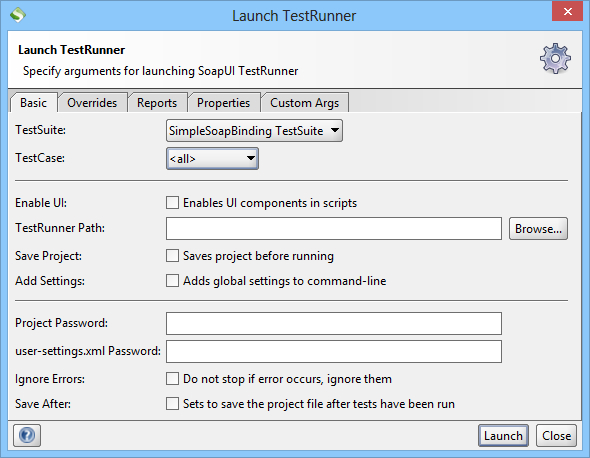
\includegraphics[width=12cm,height=12cm,keepaspectratio]{img/soapAuto.jpg}
\caption{SoapUI automation feature}
\label{overflow}
\end{figure}

The window above is SoapUI's interface for automation testing. Although it does save the tester a lot of time and reduce the chance for mistakes, it is still not completely automated in the sense that it still needs to be configured and launched manually every time. True automation requires no human efforts after the initial test case configuration.\\

One of the advantages JUnit has is that it is integrated in the Maven build process. “Apache Maven is a software project management and comprehension tool. Based on the concept of a project object model (POM), Maven can manage a project's build, reporting and documentation from a central piece of information.”\cite{maven} The VIP room web application uses Maven as its build manager. Every time a complete build (tests can be skipped to save build time) is done, the JUnit test cases are automatically run against the application. should any test fail, detail error message will be displayed in the console and the build will be marked as unsuccessful. As previously explained, JUnit “tests the smallest piece of testable software in the application.”\cite{unit} This means that JUnit test cases are likely to be static as shown by the code block on page 6. This seems to defeat the definition of functional testing, which should cover all permutation of scenario. However in software engineering, there are techniques to prove that if all single blocks are performing correctly, the entire application will work in the right way. On the other hand, there are ways connect JUnit test cases to implement a functional test case. A test controller is needed to wrap the cases to form a dynamic test. With the modified version of Simple.java and SimpleTest.java listed in the appendix, functional testing can be achieved.\\


\subsection{Reproduction}
A good testing method should have easily maintained test cases as well as simple reproduction procedure. This subsection is going to assess the easiness for an approach to save and transfer test cases between software and computers.\\

This is a criterion that causes the first approach to disqualify as a viable solution for VIP room testing. Entering data from UI cannot be recorded or saved for easy reproduction. This is why many considers this approach as a casual and informal way to do functional testing. On the other hand, both SOAP and JUnit are quite competitive in this category. SoapUI exports its test projects, which contain test suites and cases, into XML files. These XML files can be read by many other SOAP clients such as SoapSonar to import the projects. Finally, JUnit test cases are merely java files which can be transferred between testers. JUnit does fall behind in terms of compatibility. Since the test cases are so closely written to the java files that build the web application, transferring test cases can cause version control conflict and dilemma.\\

The analysis from section 3.2 and 3.3 have justified that the average time for the tester to enter data cannot be taken into account directly. The lack of automation and reproduction for approach one makes the testers who use that method spending much more time entering data than those who choose the other two approaches.


\subsection{Productivity}
This last subsection analyses how much does each approach help the tester to find defects in the code and communicate the defect to developers. This is the part that JUnit takes the leading position. Due to its deeply integrated nature, JUnit is able to detect run-time errors and unexpected outputs instantly. Moreover, the built-in error messaging and logging feature displays and saves the error neatly for developers or future testers to refer to.\\
SOAP testing does not quite have the same power as JUnit in this category. Although it is able to detect and log unexpected output through assertions, all run-time error messages are completely out of its control. Instead they depend on how the web application itself handles these errors. Most of the time a registered error message will be displayed on the SOAP client and testers will have to refer to the application's design document to find more detail in order to pin point what went wrong. Finally, the first approach has the least amount of control over these errors since not even assertions can be implemented. The tester will have to have the expected output on paper in order to determine if the output is legitimate.\\
\newpage
\section{Evaluation}
A decision matrix will be used to determine which approach is the most suitable for VIP room. 100 points will be distributed to the four criteria analysed above and the points each criterion gets will be then distributed to the three testing methods. Among the four criteria, the order of impact on efficiency is Automation (40) > Reproduction (20) = Productivity (20) > Time (15). Based on the analysis above, the final distribution is:

\begin{table}[h]\centering
\caption{Decision Matrix}
\label{dm}
\begin{tabular}{|l|l|l|l|l|l|}
\hline
      & Time & Automation & Reproduction & Productivity & Total \\ \hline
UI    & 5    & 0          & 0            & 2            & 7     \\ \hline
SOAP  & 5    & 20         & 11           & 6            & 42    \\ \hline
JUnit & 5    & 20         & 9            & 12           & 46    \\ \hline
\end{tabular}
\end{table}

\newpage
\section{Conclusions}
The decision matrix indicates that the first approach trails in almost every category while the other two competes for only a couple of points to take the lead. All three methods perform relatively similar in Time since the runtime execution time takes most part of the time measured. SOAP and JUnit splits the forty points in Automation how powerful both methods are in this category. SOAP does have a slight edge over JUnit in maintaining and reproducing because the deeply integrated nature of JUnit is losing itself points in version controlling.  However the latter was able to dominate in productivity with its great emphasis on small unit code quality which help it to secure the final lead against SOAP.\\

Although the decision is usually used to determine the best solution to a problem, it is important to notice that a quantitative value is produced as the final result. These values also shows how close each solution is with the others in terms of suitability. In this case, JUnit only beats SOAP by 4 points. This suggests that SOAP is not too bad of a solution for VIP room's testing. In fact, due to the substantially large difference in the two approaches' mechanics, it is most appropriate to use both methods at the same time. This thus can not only complement the disadvantage of both methods, but also creates redundancy to reduce the room for human error in testing.\\

\newpage
\section{Recommendations}
Based on the analysis of the three different approaches to functional testing for VIP room, this report recommends both SOAP and JUnit testing to be used as a duo testing system. This compensates both the lack of control SOAP has over the individual functions and methods and the lack of thoroughness when using JUnit. Human errors can also be kept at minimum when this redundant testing technique is present.\\

JUnit test cases should be automatically run against the application on its build process, while the SOAP test cases shall be run when the application is deployed onto the server. SOAP test cases should be carefully labelled and grouped in order for quality analysts to share. JUnit test case modifications should be severely managed by version control software. This is because of the fact that a failed JUnit test fails the build process. Unwanted changes on tests can cause many co-workers to fail in building their application locally.\\


\newpage


\addcontentsline{toc}{section}{\refname}
\bibliography{wkrpt}
\begin{thebibliography}{1}

  \bibitem{telusComp} Telus Health Inc., "Telus Health: Home," Telus Health Inc., {\em http://www.telushealth.com/} (current April 11 2014).

  \bibitem{soap} W3C Note, "Simple Object Access Protocol (SOAP) 1.1," W3C Note, {\em http://www.w3.org/TR/2000/NOTE-SOAP-20000508/} (current April 11 2014).

\bibitem{unit} Microsoft Corp., "Unit Testing," MSDN - Microsoft, {\em http://msdn.microsoft.com/en-us/library/aa292197(v=vs.71).aspx} (current April 11 2014).

\bibitem{maven} Apache Foundation., "Maven," Apache Foundation, {\em http://maven.apache.org/} (current April 11 2014).

\end{thebibliography}
\newpage


\tocsection{Acknowledgements}
I would like to thank my manager Kevin Ho and Quality Analyst Anshuman Ghandi, both of whom gave inputs on how functionality testing is done in other projects produced by Telus Health. Especially Anshuman who gave me a thorough introduction in SOAP testing and provide me with testing tools such as SoapUI and smaple test cases.\\

I would also like to thank Anna Chen, a friend of mine who inspired me to write on this topic and encouraged me to finish this report on time.\\
\newpage

\appendix{A}{Sample WSDL file}

\begin{figure}[ht!]
\centering
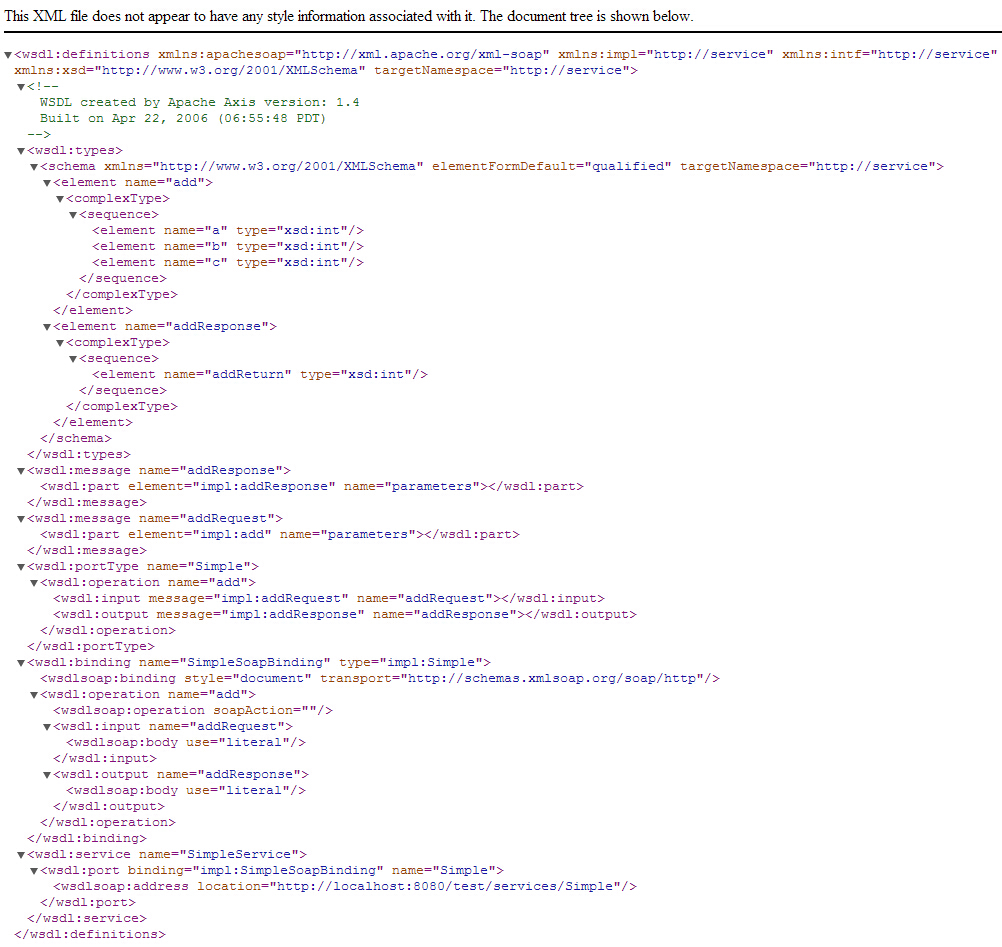
\includegraphics[width=18cm,height=18cm,keepaspectratio]{img/wsdl.jpg}
\caption{Simple.wsdl}
\label{overflow}
\end{figure}

\newpage

\appendix{B}{Simple.java}

\begin{lstlisting}
// Simple.java
public class Simple {
	public int add(int a, int b){
		return a + b;
	}
	public int subtract(int a, int b){
		return a - b;
	}
	public int multiply(int a, int b){
		return a * b;
	}
}
\end{lstlisting}

\newpage
\appendix{C}{SimpleTest.java}

\begin{lstlisting}
import static org.junit.Assert.*;
import org.junit.Test;
import service.Simple;

public class SimpleTest {
	@Test
	public void testAdd() {
		//Class Simple is being tested
		Simple tester = new Simple();
		//check if 1 3 returns 4
		assertEquals("1 + 3 must be 4", 4, tester.add(1,3));
	}
	public void testSub() {
		//Class Simple is being tested
		Simple tester = new Simple();
		//check if 8 4 returns 4
		assertEquals("8 - 4 must be 4", 4, tester.subtract(8,4));
	}
	public void testMul() {
		//Class Simple is being tested
		Simple tester = new Simple();
		//check if 2 5 returns 10
		assertEquals("2 * 5 must be 10", 10, tester.multiply(2,5));
	}
}
\end{lstlisting}

\newpage

\end{document}

